\section{Problemas de condiciones de contorno}
Se denomina problema de condiciones de contorno al conjunto de una ecuación diferencial y datos iniciales en la frontera de una región.

\subsection{Problema de Dirichlet}
El problema de Dirichlet es un problema de valores de contorno que consiste en hallar la solución $u \in C^2(\Omega)\cap C(\overline{\Omega})$ a una EDP en un dominio $\Omega$ acotado de tal forma que:
\begin{equation*}
\text{Si }
\left.
\begin{array}{l}
F\in C(\Omega)\\
f\in C(\delta\Omega)
\end{array}
\right\}
\text{Se quiere hallar } u\text{ tal que }
\left\{
\begin{array}{l r}
\mathcal{L}(u) = F &\text{en } \Omega\\
u = f &\text{en } \Omega\\
\end{array}
\right.
\end{equation*}

\subsubsection{Unicidad}
\begin{prop}{Unicidad del problema de Dirichlet}
Si $\mathcal{L}(u)=\mathcal{L}(v)$ en $\Omega$ y $u=v$ en $\delta\Omega$ entonces $u = v$ en $\Omega$.
\end{prop}
\begin{proof}
Sea $w=u-v$. Como $\mathcal{L}$ es un funcional lineal, se tiene
$$\mathcal{L}(w) = \mathcal{L}(u-v) = \mathcal{L}(u)-\mathcal{L}(v) = 0-0 = 0$$
De las hipótesis se tiene que
\begin{equation*}
\left.
\begin{array}{l l}
\mathcal{L} = 0 & \text{en } \Omega\\
w = 0 & \text{en } \delta\Omega\\
\end{array}
\right\}
\max_{\Omega}w\le\max\{0,\max_{\delta\Omega}w\} = 0
\end{equation*}
es decir, $w\le0$ en $\Omega$. Al ser $\mathcal{L}$ lineal, si $w$ es solución, $-w$ también, por tanto se puede realizar el mismo proceso para llegar a que $-w\le0$ en $\Omega$.
$$w\le0 \wedge -w\le0 \iff w = 0$$
\end{proof}


\subsubsection{Comparación de soluciones}
\begin{prop}{Comparación de soluciones}
Si $\mathcal{L}(u) \le \mathcal{L}(v)$ en $\Omega$ y $u\le v$ en $\delta\Omega$, entonces $u\le v$ en $\Omega$.
\end{prop}
\begin{proof}
Sea $w = u-v$. 
Como $\mathcal{L}$ es un funcional lineal, se tiene
$$\mathcal{L}(w) = \mathcal{L}(u-v) = \mathcal{L}(u)-\mathcal{L}(v) \le 0$$
De las hipótesis se tiene que
\begin{equation*}
\left.
\begin{array}{l l}
\mathcal{L} \le 0 & \text{en } \Omega\\
w \le 0 & \text{en } \delta\Omega\\
\end{array}
\right\}
\max_{\Omega}w\le\max\{0,\max_{\delta\Omega}w\} = 0
\end{equation*}
es decir, $w \le 0$ en $\Omega$. De donde se obtiene que $u\le v$ en $\Omega$.
\end{proof}

\subsection{Problema de Neumann}
El problema de Neumann es un problema de valores de contorno que consiste en hallar la solución $u \in C^2(\Omega)\cap C^1(\overline{\Omega})$ a una EDP en un dominio $\Omega$ acotado de tal forma que:
\begin{equation*}
\text{Si }
\left.
\begin{array}{l}
F\in C(\Omega)\\
f\in C(\delta\Omega)
\end{array}
\right\}
\text{Se quiere hallar } u\text{ tal que }
\left\{
\begin{array}{l r}
\mathcal{L}(u) = F &\text{en } \Omega\\
\frac{du}{d\nu} = f &\text{en } \Omega\\
\end{array}
\right.
\end{equation*}

\subsubsection{Unicidad}
\begin{prop}{Unicidad del problema de Neumann}
Sean $u,v$ tales que satisfacen $\mathcal{L}(u)=\mathcal{L}(v)$ en $\Omega$ y $\frac{du}{d\nu} = \frac{dv}{d\nu}$ en $\delta\Omega$.
Si $h(x)\ge0$ en $\Omega$ y en todo punto de $\delta\Omega$ se tiene la \textbf{condición de la esfera interior}, entonces $u-v=cte$ en $\Omega$.
\end{prop}
\begin{proof}
Supongamos $w=u-v\neq cte$ en $\Omega$. Al ser $\overline{\Omega}$ un compacto, o bien $w$ o bien $-w$ tiene un máximo no negativo en algún punto $x_0$. Por el principio del máximo, $x_0\in\delta\Omega$.
Por hipótesis se tiene que $\frac{dw(x_0)}{d\nu} = 0$. Sin embargo, por el \textbf{lema de Hopf} $\frac{dw(x_0)}{d\nu} > 0$. Llegamos a una contradicción al suponer que $w=u-v\neq cte$ en $\Omega$.
\end{proof}
\see
\noindent Si $h(x) > 0$ en algún punto de $x\in\Omega$, entonces $u=v$.

\noindent Como $\mathcal{L}(u-v) = 0$, se tiene
$$\mathcal{L}(u-v) = -\Delta (u-v) + \sum_{i=1}^n g_i(x)\frac{d(u-v)}{dx_i} + h(x)(u-v) = 0$$
Pero $u-v=cte$, por lo que queda que
$$h(x)(u-v) = 0$$ Como $h(x)$ es estrictamente positiva, entonces $u-v=0$.

\example
Vamos a ver la necesidad de que $h(x)\ge 0$ en todo el dominio.
Se tiene la ecuación siguiente:
$$-u''-u=0$$
en la que $h(x) = -1 < 0$.
Dos soluciones de esta ecuación son
\begin{equation*}
\begin{array}{l}
u_1(x) = sin(x)\\
u_2(x) = cos(x)\\
\end{array}
\end{equation*}

\begin{figure}[ht]
\centering
\begin{subfigure}{.5\textwidth}
	\centering
  	\begin{tikzpicture}
		\draw[->] (-0.5,0) -- (4,0) node[right] {$x$};
		\draw[->] (0,-1) -- (0,1.5) node[above] {$y$};
		\draw[-] (pi/2,0.1) -- (pi/2,-0.1) node[below] {$\frac{\pi}{2}$};
		\draw[-] (pi,0.1) -- (pi,-0.1) node[below] {$\pi$};
		\draw[] (-0.2,0) node[below] {$0$};
		\draw[fill, blue] (pi/2, 1) circle[radius=0.5mm];
		\draw[scale=1,domain=0:pi,smooth,variable=\x,blue] 
			plot ({\x},{sin(\x r)})
			node[above right] {$u(x)$};
	\end{tikzpicture}
	\caption{$u(x) = sin(x)$}
	\label{fig:sol-contraejemplo-h1}
\end{subfigure}%
\begin{subfigure}{.5\textwidth}
	\centering
  	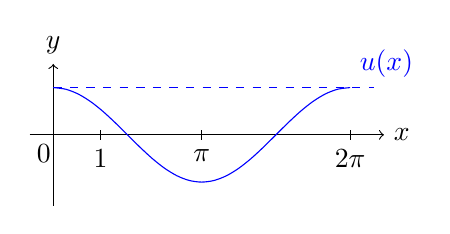
\begin{tikzpicture}[scale=0.6]
		\draw[->] (-0.5,0) -- (7,0) node[right] {$x$};
		\draw[->] (0,-1.5) -- (0,1.5) node[above] {$y$};
		\draw[-] (pi,0.1) -- (pi,-0.1) node[below] {$\pi$};
		\draw[-] (2*pi,0.1) -- (2*pi,-0.1) node[below] {$2\pi$};
		\draw[-, dashed, blue] (0,1) -- (2*pi+0.5,1);
		\draw[] (-0.2,0) node[below] {$0$};
		\draw[-] (1,0.1) -- (1,-0.1) node[below] {$1$};
		\draw[scale=1,domain=0:2*pi,smooth,variable=\x,blue] 
			plot ({\x},{cos(\x r)})
			node[above right] {$u(x)$};
	\end{tikzpicture}
	\caption{$u(x) = cos(x)$}
	\label{fig:sol-contraejemplo-h2}
\end{subfigure}%
\caption{Funciones periódicas}
\label{fig:sol-contraejemplo-h}
\end{figure}

\noindent En la figura \ref{fig:sol-contraejemplo-h1} se puede ver como se alcanza un máximo no negativo en el interior del invervalo. En la figura \ref{fig:sol-contraejemplo-h2} se observa como la función llega a los extremos del intervalo con derivada nula. Ambas situaciones se deben a que no se cumple la condición $h(x) \ge 0$.

\example
Vamos a ver la necesidad de que $\Omega$ sea un dominio acotado.
Sean $u(x,y) = e^xsin(x)$ y $\Omega = \mathbb{R}\times(0, \pi)$
Se tiene que 
\begin{equation*}
u \text{ cumple}
\left\{
\begin{array}{l l}
-\Delta u = 0 & \text{en }\Omega\\
u=0 & \text{en } \delta\Omega\\
\end{array}
\right.
\end{equation*}
\begin{equation*}
\delta\Omega = (\mathbb{R}\times\{0\})\cup(\mathbb{R}\times\{\pi\})
\end{equation*}
Dado que $u(x) = 0$ en toda la frontera, se tiene que cumplir que $u(x) \le 0$ en $\Omega$, sin embargo, esto es falso por no ser $\Omega$ acotado (ver figura \ref{fig:u3d1}).

\begin{figure}[ht]
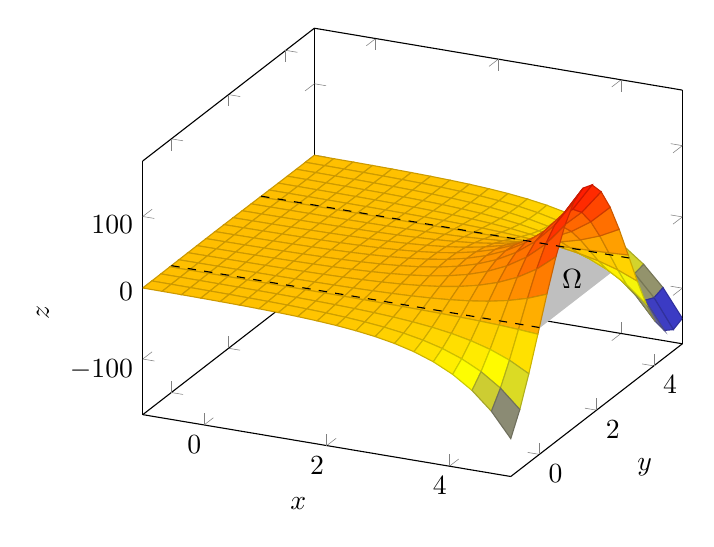
\begin{tikzpicture}
\begin{axis}[
	xlabel=$x$,
	ylabel=$y$,
	zlabel=$z$
]

\addplot3 [color=lightgray, fill] coordinates {(-1,pi,0) (5,pi,0) (5,0,0) (-1,0,0)};

\addplot3[
	surf,
    domain=-1:5,
    samples=20,
	] {(exp(\x))*sin(\y r)};

\addplot3 [color=black, dashed] coordinates {(-1,0,0) (5,0,0)};
\addplot3 [color=black, dashed] coordinates {(-1,pi,0) (5,pi,0)};
\node at (axis cs:4.6,2,0) {$\Omega$};
\end{axis}
\end{tikzpicture}
\caption{$u(x,y) = e^xsin(y)$}
\label{fig:u3d1}
\end{figure}

\newpage
\subsection{Principio débil del máximo dado por una función F}
\begin{theorem}
Sea $\Omega$ un dominio acotado, $u\in C^2(\Omega)\cap C(\overline{\Omega})$. 
Sea la inecuación
$$\mathcal{L}(u) \le F  \text{ en } \Omega\\$$
Si $g_1,\hdots,g_n,h,F$ son acotadas y $h(x) \ge 0$ entonces,
$$u(x) \le \max\{0, \max_{\delta\Omega}u\} + C\max\{0, \max_{\Omega} F\}$$
con $C$ una constante que depende del dominio $\Omega$ y de $g_1,\hdots,g_n$.
\end{theorem}
\begin{proof}
Se va a denotar
\begin{equation*}
\left\{
\begin{array}{l}
\mathcal{L}_0(u)=-\Delta u+\sum_{i=0}^ng_i(x)\frac{du}{dx_i}\\
\mathcal{L}(u) = \mathcal{L}_0(u)+h(x)u\\
M=\max\{0,\max_{\delta\Omega}u\}
\end{array}
\right.
\end{equation*}
Dado que $\Omega$ es un dominio acotado, se tiene que
$\Omega\subset\{x\in\mathbb{R}^n: 0<x_1<d\}$ para algún $d\in\mathbb{R}$.
Definimos $\varphi(x)$ siendo $K$ una constante positiva.
$$\varphi(x)=K\left(e^{\alpha d}-e^{\alpha x_1}\right)+M > M \ge 0$$
Calculamos $\mathcal{L}_0(\varphi)$:
$$\mathcal{L}_0(\varphi)=-Ke^{\alpha x_1}\{-\alpha^2+\alpha \underbrace{g_1(x)}_{\text{acotada}}\}>Ke^{\alpha x_1} > K > 0$$
si tomamos un valor de $\alpha$ lo suficientemente grande.

\noindent Definimos ahora $w=u-\varphi$ y calculamos $\mathcal{L}(w)$:
$$\mathcal{L}(w) = \mathcal{L}(u)-\mathcal{L}(\varphi) \le F - \mathcal{L}_0(\varphi)-\underbrace{h(x)\varphi(x)}_{\ge0}<F(x)-K \le 0$$
Basta tomar $K=\max\{0, \max_{\Omega}F\}$ para tener $\mathcal{L}(w) < 0$.
Por otro lado se tiene que $u\le M$, por tanto $u-\varphi\le M - M = 0$. Es decir, $u \le \varphi$. Entonces 
$$u_\Omega \le \varphi_\Omega\implies u_\Omega \le K\max_\Omega\left(e^{\alpha d}-e^{\alpha x_1}\right) + M = K\left(e^{\alpha d}-1\right) + M$$
\textbf{Conclusión:}

Denotamos $C = \left(e^{\alpha d}-1\right)$. Se puede observar que $C$ depende de $\alpha$ y $d$, es decir, que depende ensencialmente del dominio y de la cota de las funciones $g_1,\hdots,g_n$.
Se tiene entonces que 
$$u(x) \le \max\{0, \max_{\delta\Omega}u\} + C\max\{0, \max_{\Omega} F\}$$
\end{proof}

\corol
Para $\mathcal{L}(u) = F$ en $\Omega$ se tiene
$$
\sup_{\Omega}|u| \le \sup_{\delta\Omega}|u|+C\sup_\Omega |F|
$$
\begin{proof}
En principio se tiene
\begin{equation}\label{eq:corol-2-1-1}
\sup_{\Omega}(u) \le \max\{0, \max_{\delta\Omega}(u)\}+C\max\{0,\max_\Omega (F)\}
\end{equation}

Por otro lado, si $\mathcal{L}(u) = F$, al ser $\mathcal{L}$ lineal se tiene que $\mathcal{L}(-u) = -\mathcal{L}(u) = -F$. Por tanto se cumple 
\begin{equation}\label{eq:corol-2-1-2}
\sup_{\Omega}(-u) \le \max\{0, \max_{\delta\Omega}(-u)\}+C\max\{0, \max_\Omega (-F)\}
\end{equation}
A partir de \eqref{eq:corol-2-1-1} y \eqref{eq:corol-2-1-2} se obtiene el resultado.
\end{proof}

\newpage
\subsection{Dependencia continua de los datos}
\begin{prop}{Dependencia continua de los datos para el problema de Dirichlet}
Supongamos $u_1, u_2$ satisface 
\begin{equation*}
\left.
\begin{array}{l l}
\mathcal{L}(u_i)=F_i & \text{en } \Omega\\
u_i=f_i & \text{en } \delta\Omega\\
\end{array}
\right\} (i=1,2)
\end{equation*}
Se tiene que, siendo $C$ una constante:
$$\sup_\Omega|u_1-u_2| \le \sup_{\delta\Omega}|f_1-f_2|+C\sup_\Omega|F_1-F_2|$$
\end{prop}
\begin{proof}
Basta aplicar el corolario anterior tomando
\begin{equation*}
\left.
\begin{array}{l l}
\mathcal{L}(v)=F_1-F_2 & \text{en } \Omega\\
v=f_1-f_2 & \text{en } \delta\Omega\\
\end{array}
\right\} (i=1,2)
\end{equation*}
\end{proof}

\subsection{Problema bien propuesto}
\begin{definition}{Problema bien propuesto}
Diremos que un problema está bien definido o bien propuesto (en el sentido de Hadamard), si la solución
\begin{itemize}
\item existe
\item es única
\item hay dependencia continua respecto de los datos
\end{itemize}
\end{definition}